\chapter{Introduction}
\label{ch:introduction}

\section{Rationale and motivation of the thesis}

Glacier ice melts due to various heat inputs, and when the resultant meltwater is naturally dammed by ice, moraine, or bedrock, glacial lakes can form in various locations relative to the glacier. These locations are on the surface of the glacier (and the lake is called supraglacial), within the glacier (englacial), beneath the glacier (subglacial), at the glacier's margin (ice-marginal), or dammed by a moraine or the bedrock beyond the glacier's terminus (proglacial). Presently, over 110,000 glacial lakes are reported worldwide, covering a total area of  $\approx$15,000 km$^2$ (\cite{Zhang&al2024}, see Fig.~\ref{fig:fig1_zhnagetal2024}). Glacial lakes are the most present in Greenland, the Southern Andes, Antarctica, Alaska, Canada, and High Mountain Asia \citep{Shugar&al2020}. The primary concern of glacial lakes is the potential hazards they pose, and not their contribution to sea level rise as glacial lakes hold about 0.43 mm of sea level equivalent \citep{Shugar&al2020}. 

Glacial outburst floods are sudden releases of water from a glacier. When this water originates from a lake, the events are referred to as glacial lake outburst floods (GLOFs). GLOFs occur when the dam containing a glacial lake fails due to various triggers, which depend on the type of dam. GLOFs are infrequent but high-magnitude events with substantial geomorphic consequences such as erosion, sediment transport, and landscape alteration \citep[e.g.][]{Cook&al2018}. In particular, GLOFs pose serious threats to human lives and infrastructure in high mountain regions. A world-wide documentation of 1,348 GLOFs show that 24\% of them have recorded societal impacts \citep{Carrivick&Tweed2016}. This study records 7 deaths in Iceland, 393 in the European Alps, 5745 in South America, and 6300 in Central Asia. Notable events include the 1941 GLOF in Huaraz, Peru, which destroyed a third of the city and killed about 5000 people \citep{Carey2005}, and the 2013 GLOF in Kedarnath, India, which resulted in over 6000 deaths \citep{Allen&al2016}. The GLOFs inventory first compiled by \cite{Carrivick&Tweed2016} was further extended by \cite{Emmer&al2022, Veh&al2022, Lutzow&al2023} to 3000 GLOFs reported worldwide from 850 to 2022. Most GLOFs occurred in Alaska (24\,\%), High Mountain Asia (18\,\%) and Iceland (19\,\%), the majority (64.8\,\%) being from ice-dammed lakes. Recorded GLOFs have increased in most glaciated mountain regions worldwide, with ongoing deglaciation and lake expansion expected to further increase their frequency, in particular for glacial lakes dammed by frontal moraine \citep{Harrison&al2018,Zhang&al2024}. It is estimated that over 15 million people are currently at risk from GLOFs, primarily due to dam failures or wave overtopping caused by mass movements falling into the lake in the Himalayas and Andes \citep{Taylor&al2023}. However, note that this study considers populations at risk if they are located in less than 1\,km from a river originating from a glacial lake, within a distance of 50\,km. This approach may overestimates the number of people threatened by small glacial lakes, as GLOFs from these lakes don't reach as far. %Consequently, the number of people threaten may be overestimated in the Alps, where relatively small, stable glacial lakes have minimal impact, although located in densely populated regions (e.g. the bedrock-dammed lake of Rhoneglestcher in the Rhone valley). 
The European Alps are the most susceptible region worldwide for GLOFs with 443 events ever recorded in 89 sites since 1560 \citep{Carrivick&Tweed2016,Lutzow&al2023}. However, the fact that GLOFs have been overlooked in the European Alps compared to other regions of the world may explain these results \citep{Veh&al2022}. In Switzerland, more than 200 GLOFs were recorded for 60 sites since 1560 \citep{Carrivick&Tweed2016}. Approximately 30-40\,\% of these glacial outburst floods were estimated to originate from englacial and subglacial water reservoirs known as water pockets, rather than from identified lakes \citep{Haeberli1983}. In general, very little is known about water pockets due to their hidden nature, despite them being responsible for a significant proportion of outburst events 

Given the widespread risk posed by GLOFs, particularly in a warming climate and in densely populated areas such as the European Alps, it is crucial to understand the formation, evolution, and physical characteristics of glacial lakes to predict their magnitude and mitigate their impacts on downstream communities and infrastructure. In this regard, research on GLOFs has been considerably increasing in the last years. For instance, \cite{Emmer&al2022} reported a 110\,\% increase in the number of peer-reviewed scientific publication on GLOFs between 2017 and 2021. However, this is largely due from advancements in remote sensing capabilities and most of our fundamental understanding of GLOFs mechanisms comes from earlier studies \citep[see][for a review]{Bjornsson2010}.

The current limited physical understanding of some type of GLOFs prevent their prediction for natural hazard purposes \citep{Emmer&al2022}. This is particularly the case for the drainage of supraglacial lakes \citep[e.g.][]{Vincent&al2010} and the outburst flood originating from water pocket \citep[e.g.][]{Haeberli1983}. In both type of floods, the lack of field measurements prevent robust modelling framework and thus further accurate predictability of their occurrence and impacts. This general lack of detailed field measurement and physical understanding on GLOFs is identified in numerous recent studies \citep{Zhang&al2024, Carrivick&Tweed2016, Veh&al2022}.

In this thesis, I aim to contribute to the understanding of glacial outburst floods by providing 1) an extensive field-based dataset of an ice-marginal lake drainage at the glacier surface constraining some important physical parameters, 2) an up-to-date inventory of glacial outburst floods originating from water pockets in alpine glaciers and insights on their mechanisms, and 3) insights on the limitation of monitoring technique such as the ground penetrating radar for the detection of englacial water pockets. Each of these listed points are analyzed in a dedicated chapter corresponding to a published (or submitted) peer-reviewed article.


\section{Glacier outburst floods: current understanding and research gaps} 

The characteristics of GLOFs, such as the triggering process, the magnitude, the mechanisms of drainage and the impacts downstream depend on the type of lake and dam from which they originate. Therefore, differentiating type of GLOFs by the type of the dam constitutes the first step for GLOFs hazard assessment \citep{Allen&al2022}. Here, we classify glacier outburst floods according to the type of water reservoir they originate from, i.e., from moraine-dammed lakes, bedrock-dammed lakes, ice-dammed lakes (also called ice-marginal lakes), subglacial lakes, water pocket, and supraglacial lakes. Note that even in recent studies \citep[e.g.][]{Lutzow&al2023,Zhang&al2024} these different categories are not clear. Refer to Table~\ref{tab:glof_types} for clarification on the different types of lakes as defined in three review studies \citep{Roberts2005,Lutzow&al2023,Zhang&al2024}, and for their corresponding glacier outburst floods. In this section, we mirror the type of glacier outburst floods corresponding to theses type of lake. For each of these categories, we review the current knowledge on their spatial and temporal distribution, on the rupture mechanisms at play, on their flood modelling and on the challenges associated. 


\begin{table}[ht]
\caption{Examples of lake types and glacier outburst floods associated as defined in the literature. GLOFs stands for glacial lake outburst floods. WPOFs stands for water pocket outburst floods.}
\centering
\small
\begin{tabular}{l l l |l}
\hline
\textbf{Type of lake} & & & \textbf{Type of glacier}\\
\textbf{in {\cite{Roberts2005}}} & \textbf{in {\cite{Zhang&al2024}}} & \textbf{in {\cite{Lutzow&al2023}}} & \textbf{outburst floods} \\
\hline
1. Ice-marginal, &  ice-dammed & ice-dammed & GLOFs,\\
ice-dammed &  &  & jökulhlaups  \\
 & & & {\citep{Bjornsson2010}}\\
\hline
2. Supraglacial & supraglacial & ice-dammed &  GLOFs\\
\hline
3. Volcanic  & other & volcanic & GLOFs, \\
 &  &  & jökulhlaups \\
 & & &  {\citep{Bjornsson2010}}\\
\hline
4. Subglacial & other & ice-dammed & GLOFs,\\
 &  &  & jökulhlaups  \\
 & & & {\citep{Bjornsson2010}}\\
\hline
5. Intraglacial cavity & englacial & water pocket & WPOFs \\
  &  &  & {\citep{Deline&al2004}}, \\
& & & GLOFs \\
& & & {\citep{Lutzow&al2023}}\\
& & & {\citep{Zhang&al2024}}\\
\hline
6. Moraine-dammed & moraine-dammed & moraine-dammed & GLOFs \\
 & bedrock-dammed & bedrock-dammed &  GLOFs \\
\hline
7. Surge termination & not specified & not specified & GLOFs\\ %{\cite{Kamb&al1985}}\\
\hline
\end{tabular}
\label{tab:glof_types}
\end{table}

\begin{figure}
    \centering
    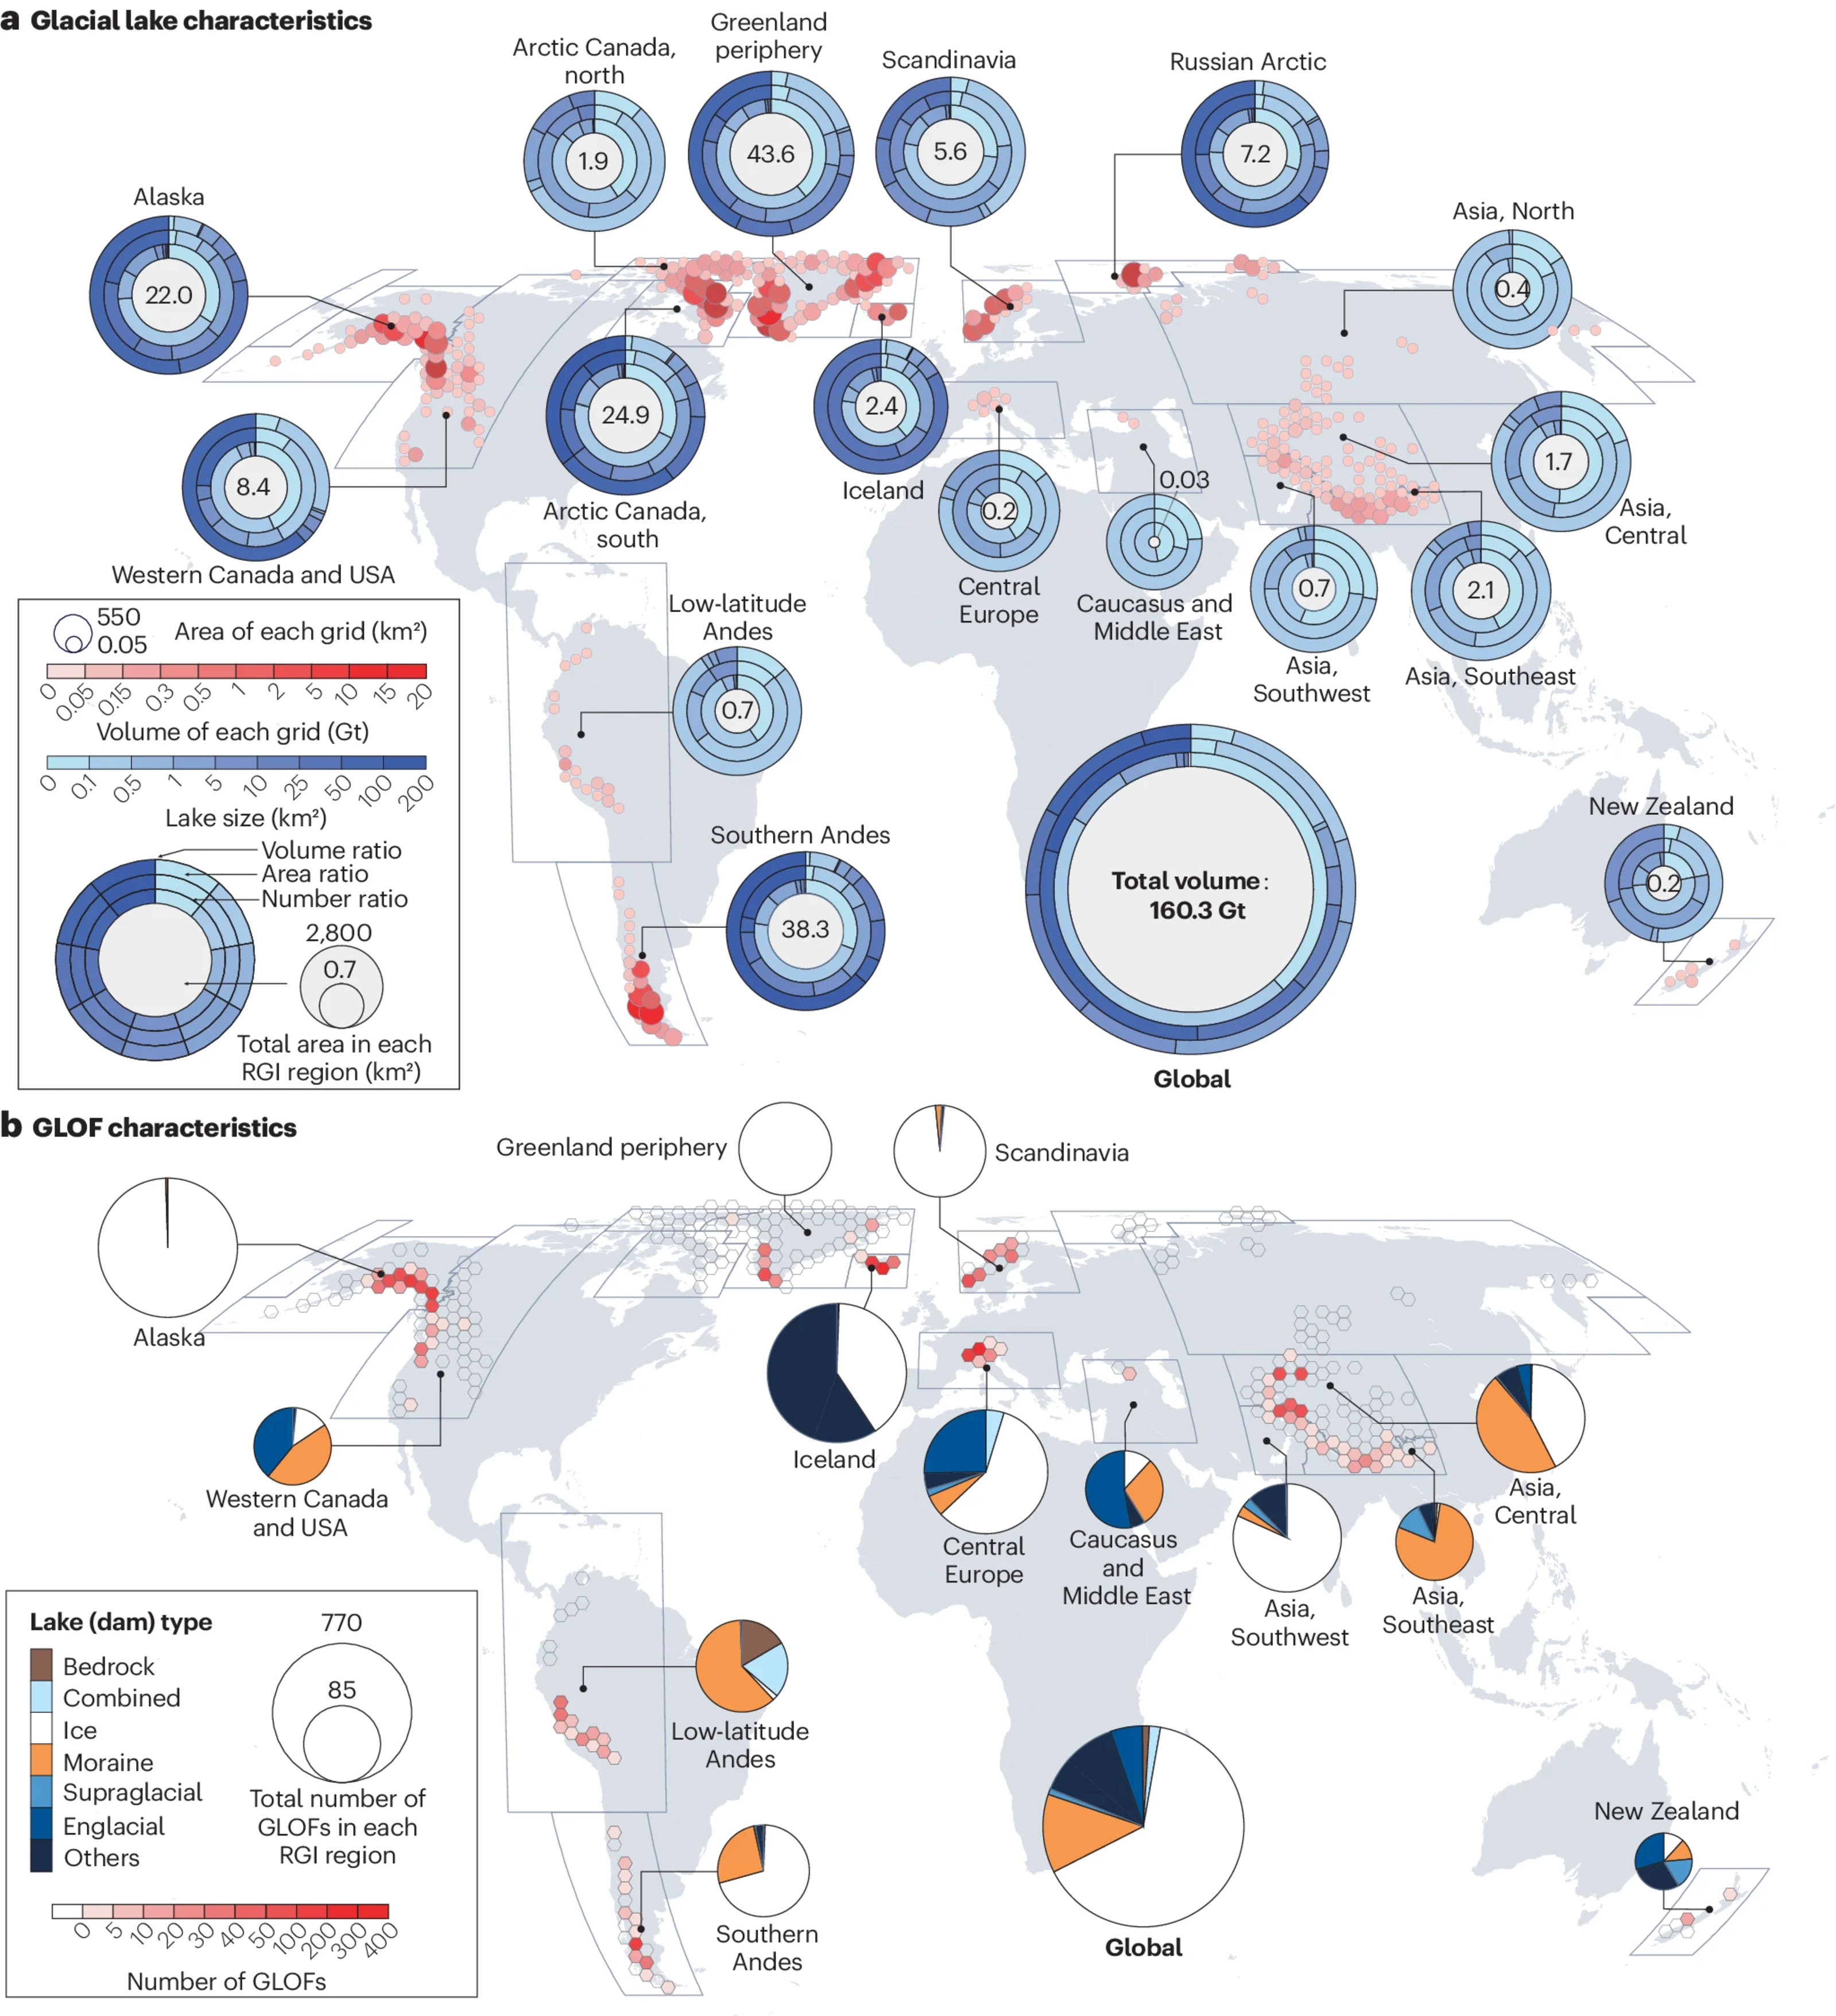
\includegraphics[width=1\linewidth]{chapters/introduction/Fig1_Zhnag&al2024.pdf}
    \caption{From \cite{Zhang&al2024} (with permission). a) Area and volume of present-day (2018) glacial lakes within 1\,km of glaciers, aggregated over 220\,km hexagon grid cells (red shades), and regional statistics of lake volume, area and number according to Global Terrestrial Network for Glaciers (GTN-G) glacier regions of the Randolph Glacier Inventory (RGI)(doughnut plots); outer, middle and inner circles indicate the total volume, area and number percentage of glacial lakes in a given size interval, respectively, with the total lake area in each region in the centre of the circle. b) Global distribution of historical glacial lake outburst floods (GLOFs) aggregated over 220\,km hexagon grid cells (red shading), and regional breakdown of the GLOF number by glacial lake (dam) types (pie charts).}
    \label{fig:fig1_zhnagetal2024}
\end{figure}


\subsection{GLOFs from moraine-dammed lakes and bedrock-dammed lakes}% pro glacial lakes
% also see Carriveek and tweed 2015 if more material needed  https://doi.org/10.1111/gto.12094

Moraine-dammed lake are impounded by the frontal moraine and the glacier front. Moraine dam breaching can be caused by seepage of lake water through unconsolidated material, degradation of an ice core, or overtopping due to calving, avalanches or landslides into the lake \citep{Tweed&Russel1999,Emmer&al2022}. GLOFs from moraine-dammed lakes constitute 13\,\% of all documented outbursts globally \citep{Lutzow&al2023}. Their occurrence varies regionally (see Fig.~\ref{fig:fig1_zhnagetal2024}, with most cases reported in the low-latitude Andes (n=100; 61.3\,\% of GLOFs within the low-latitude Andes, 25.1\% of global moraine-dammed GLOFs), Central Asia (n=110; 46.2\,\% of GLOFs in central Asia, 27.6\,\% of global moraine-dammed GLOFs), and the Himalaya (n=71; 77.2\,\% of GLOFs in the Himalaya, 17.8\,\% of global moraine-dammed GLOFs). GLOFs from moraine-dammed are expected to occur more frequently in the next decades and into the 22$^{nd}$ century in response to climate warming \citep{Harrison&al2018}. In Switzerland, for instance, the count of moraine-dammed lakes increased from 21 in 1900 to 47 in 2006, and then to 82 in 2016 \citep{Zhang&al2024}. However, some of this increase is due to the artificial impoundment of lakes by dams for hydropower generation, as most moraine-dammed lakes susceptible to breach from past moraines have already been breached in the European Alps (i.e.\ moraines that formed during the little ice age which occurred between 1300 to 1850). Therefore, this increase may not be directly relevant to the hazard posed by GLOFs. %Complete failure of the (moraine) dam restricts any future ability to impound meltwater \citep{Clague&Evans2000}. Hence, moraine-dammed lakes usually fail only once. % In \cite{Zhang&al2024}: 
% Moraine-dammed lakes in the ice-marginal phase of evolution are the most likely to pro-duce GLOFs due to calving processes and proximity to ice avalanche release zones. In contrast, glacial lakes detached from glaciers become disconnected from the most frequent GLOF-triggering processes with increasing distance from glaciers [56]. 
Since moraine-dammed lake are well visible and their area is relatively easily measurable (e.g. from remote sensing technique), it is relevant to assess their flood potential from their size. Empirical relationships between peak discharge, water volume and water height has been established to predict the flood magnitude \citep[see][for a review on moraine-dammed lake failure]{Neupane&al2019}. Recent improvement on the prediction of flood magnitude considered solid particles dynamics in modelling studies \citep[e.g.][]{Mergili&al2018}. However, very limited experimental investigations have been conducted on the failure mechanism of moraine dams, and the cascade effect of moraine dam failures remains poorly know \citep{Somos-Valenzuelas&al2016}. This currently limits the understanding of moraine failure mechanism and their downstream impacts \citep{Neupane&al2019}. 

%modelling of moraine dam failure: https://doi.org/10.5194/esurf-3-171-2015
%mass movement into proglacial lakes: Haeberli 2017

Bedrock-dammed lakes form when solid bedrock acts as a barrier to impound water near the glacier. Unlike moraine dams, bedrock dams are relatively stable and less prone to failure because of the robustness of the bedrock barrier. Consequently, GLOFs from bedrock-dammed lakes typically occur only when the dam is overtopped by mass movement into the lake, such as landslides, rockfalls or ice and snow avalanches \citep{Huggel&al2004, Haeberli&al2017,Emmer2017}. These events constitute only $\approx$1\,\% (30 out of 3151) of the total documented GLOFs in \cite{Lutzow&al2023} (see also Fig.~\ref{fig:fig1_zhnagetal2024}).


\subsection{GLOFs from ice-dammed marginal lakes}
\label{subsection:glofs_ice-dammed_lakes}

Ice-dammed marginal lakes form when thick glaciers block the flow of water, creating a natural dam that temporarily impounds water at the glacier's margins. Note that in \cite{Lutzow&al2023,Zhang&al2024}, ice-dammed marginal lakes are simply called ice-dammed lake, but we add marginal to differentiate more explicitly with supraglacial lakes, subglacial lake and englacial water pocket in the next subsections, which are also reservoir of water dammed by ice. GLOFs from ice-dammed marginal lakes \citep[also called  jökulhlaups in][]{Bjornsson2010} occur when the ice dam fails by hydrofracturing due to the lake's hydrostatic pressure \citep[e.g. in][]{Lindner&al2020}, subglacial channel enlargement \citep{Nye1976} or ice dam flotation \citep[e.g. in][]{Liestol1956}, or a combination thereof \citep{Flowers&al2004}\citep[see also][for a review on the physical aspects of these mechanisms]{Flowers2015}. Alternatively, the lake water can overspill the dam and forms a breach due to ice erosion \citep[e.g.][]{Walder&Costa1996,Raymond&Nolan2000,Mayer&Schuler2005}. Glacial lake outburst floods originating from ice-dammed marginal lakes are the most prevalent type of all type of GLOFs, accounting for 64.8\,\% of occurrences worldwide (see Fig.~\ref{fig:fig1_zhnagetal2024}). At the regional scale, Alaska has the most GLOFs from ice-dammed marginal lakes (n = 764; 99\,\% within Alaska, 37\,\% of global ice-dammed GLOFs) \citep{Emmer&al2022}. Ice-dammed marginal lakes are also the main source of GLOFs in Greenland periphery (n = 153; 100\,\% within Greenland, 7.5\,\% globally), the Karakoram (n = 190; 33.4\,\% within HMA, 9.3\,\% globally), Scandinavia (n = 183; 96.8\,\% within Scandinavia, 9.0\,\% globally), Central Europe (n = 258; 58.2\,\% within Central Europe, 12.7\,\% globally), and Iceland (n = 237; 40.2\,\% within Iceland, 11.6\,\% globally)\citep{Zhang&al2024}. The high frequency of GLOFs from ice-dammed marginal lakes is attributed to the possibility of multiple draining events, because the ice dam can temporarily "re-heal" once a large part of the lake water had been drained \citep{Zhang&al2024}. Despite some current positive trends, declining trends in ice-dam failures may dominate in the future due to ongoing ice loss preventing the formation of such dams \citep{Rick&al2022}. As glaciers retreat, many glacier dams become unable to impound lakes at higher elevations due to steeper topography \citep{Zhang&al2024}, or the glaciers disappear entirely \citep[e.g.][]{Tweed&Russel1999,Geertsema&Clague2005}. %former part because we don't want to arise question we don't answer:
%However, the decrease in ice-dammed lakes does not necessarily correlates with a decrease in GLOFs. For instance, in Alaska, the total number and area of ice-dammed lakes decreased by 13\,\% and 43\,\%, respectively, between 1984 and 2019 because of glacier recession \citep{Rick&al2022}. Nevertheless, there was an increase in GLOFs for the same period, indicating that the regional increases in ice-dammed failures are linked to fewer lakes emptying more frequently \citep{Veh&al2022}, but to my knowledge the causes were not resolved in the mentioned studies.

When predicting the impact of a GLOF downstream, the peak discharge and the hydrograph (i.e., the discharge time series of the flood) are of particular interest. The flood peak discharge can be estimated using empirical relationships between the lake area and the lake volume \citep{Evans1986, Huggel&al2002, Cook&Quincey2015}, and then between the lake volume and the peak discharge \citep{Clague&Mathews1973, Haeberli1983, Costa1985, Evans1986, Walder&OConnor1997, Huggel&al2002}, although these empirical formulations have shown limitations \citep[e.g.][]{Huss&al2007}. Flood hydrographs, however, need a physical-based calculation to be accurately modeled. In particular, the hydraulics and the thermodynamics of the water flow through the ice has to be considered. The understanding of jökulhlaups hydraulics was significantly advanced by the development of the general theory of time-dependent turbulent water flow through intraglacial conduits by \cite{Nye1976}, who build his work on \cite{Roethlisberger1972,Shreve1972,Weertman1972}. This theory explains flood evolution by considering water input at the upper end of a ice tunnel from a reservoir, accounting for the heat stored in the lake and the tunnel's geometry. According to these studies, the lake drainage can start when the lake hydrostatic pressure lead the dam to float. The tunnel grows due to positive feedback, with the ice walls melting from the frictional heat generated by the flowing water, leading to increasing discharge. The flood discharge is then controlled by the lake level (which determines the hydraulic gradient) and the changes in channel size. Theses changes are linked to the melting rates at the channel walls, driven by the dissipation of potential energy. This jökulhlaups model from \cite{Nye1976} was refined by \cite{Spring&Hutter1981} and \cite{Clarke1982} to incorporate water reservoir temperatures, heat transfer in the tunnel, and the geometry of both the lake and the subglacial pathway. This model was further improved by \cite{Clarke2003} by using field data from Grímsvötn outbursts in Iceland \citep[see][]{Bjornsson2010}. These improvements considered that the location of flow constrictions, which control the flood's magnitude, may shift upward along the flood path. To summarize, by the end of the twentieth century, our understanding of ice-dammed marginal lake drainage mainly came from observed jökulhlaups in Iceland, which provided detailed datasets including water temperature, lake level variations and hydrograph of the flood. Despite these advancements, certain model parameters necessary for accurately modeling jökulhlaups and reconstructing flood hydrographs remained poorly constrained.

The need for field-based observation to better calibrate jökulhlaup models was highlighted in \cite{Clarke2003}. In particular, the author found the previous estimate of flow resistance in the ice tunnel were suggested to be too high, and that the empirical formulas of heat exchange between ice and water were possibly inappropriate. In addition, the observed discharge characteristics of a significant jökulhlaups from Grímsvötn in Iceland, as described by \cite{Bjornsson1996}, could only be explained by integrating subglacial flow through both a sheet and conduits \citep{Flowers&al2004}. This model suggests that pressurized floodwater initially propagates in a turbulent subglacial sheet before transitioning to conduits having higher streamflow discharge capacity. However, simulated outlet water temperature was overestimated, emphasizing a persistent discrepancy between observations and the predictions of jökulhlaups thermodynamic theory \citep[as already indicated by ][]{Clarke2003}. Although these discrepancies between observed and modeled water temperatures at the outlet did not significantly affect the simulation results in \cite{Flowers&al2004}, they indicate that more work is needed on the heat exchange parametrization for accurate simulations of jökulhlaups. 

In recent years, ice-dammed marginal lake drainages had been monitored in Alaska \citep[Hidden Creek Lake, ][]{Anderson&al2003,Anderson&al2005,Walder&al2005,Walder&al2006}, Switzerland \citep{Huss&al2007, Werder&al2010} and Yukon \citep{Bigelow&al2020}. However, none of these studies included temperature measurements, which prevented to characterize the thermodynamics of their drainage. 
%In \cite{Huss&al2007}, the GLOF from the ice-marginal lake Gornersee was monitored in detail for two years. Measurements included lake geometry, water pressure in nearby boreholes, glacier surface motion. In addition, input and output lake discharge were modeled. Results show that, even within a single lake system, various drainage processes lead to various hydrograph. This study highlights the need for an integrative assessment of glacier-dammed lake floods to better understand these events. 
While the study of Gornersee in \cite{Huss&al2007} validated the proportionality of the empirical relationship of \cite{Clague&Mathews1973} regarding the peak discharge and the lake volume, it found that peak discharges of the lake outburst were significantly below the values predicted by this empirical relation. \cite{Werder&al2010} attempted to model the hydrograph of an ice-marginal lake at Unterer Grindelwaldgletscher based on field data previously acquired. However, too little constrain on the choice of the channel roughness value (i.e. the resistance of the water flow) led to large uncertainties on the peak discharge. The additional and recent theoretical work on the heat transfer between water and ice in \cite{Sommers&Rajaram2020} showed the importance in considering the stream flow geometry (e.g. wide sheet or circular channels) on the heat transfer parametrization. The results of this study could explain part of the temperature discrepancies between observation and jökulhlaups models highlighted in \cite{Clarke2003,Flowers&al2004}. The heat exchange between the ice and water flows is a important parameter that partly controls the evolution of the subglacial channel size and, consequently, the outflow from the lake. Yet, in situ field measurements are still needed to validate our understanding of how this heat exchange impacts ice-dammed lakes drainage.

% in parrallell, recent model couple the subglacial fllod routing to the ice dynamics (Kingslake and Ng 2013, Kingslake 2015, Pimentel and flowers 2010 (https://doi.org/10.1098/rspa.2010.0211)
% potential adding: Kingslake and Ng 2013 -> assess modeling performance on the prediction of the timing of an ice-marginal lake GLOFs in Kyrghistan -> Local predictions of the occurrence and timing of GLOFs from temperature data alone have been only partly successful

\subsection{GLOFs from subglacial lakes}
\label{subsection:glofs_subglacial_lakes}

% Lakes at the glacier base, i.e.\ subglacial lakes, are dammed by the ice until that the hydrostatic pressure of the lake water reaches the ice dam flotation and leads to the drainage of the reservoir \citep[e.g.][]{Bjornsson2010}. The drainage can also be initiated through pre-existing veins and channels that are progressively enlarged \citep{Nye1976}. Note that subglacial lakes are usually caused by heat fluxes at the glacier base and are more common in ice sheets or in ice caps associated to geothermal activities, rather than in Alpine glaciers \citep{Livingstone&al2022}. 

Subglacial lakes are formed by volcanic activity or geothermal flux at the glacier base in addition to surface melt, and are impounded by the glacier ice. GLOFs from subglacial lake occur when the hydrostatic water pressure overcome the ice overburden pressure and/or subglacial channels enlarge by positive feedback (see the previous subsection GLOFs from ice-dammed marginal lakes for details of the subglacial drainage mechanisms). Note that GLOFs originating from subglacial lakes are also referred to as jökulhaups in \cite{Bjornsson2010}, similar to GLOFs resulting from ice-dammed marginal lakes, as they involve similar rupture mechanisms. Relatively few GLOFs are attributed to subglacial lakes induced by geothermal or volcanic activity (8\,\%) compared to other triggers and mechanisms \citep{Lutzow&al2023}. The majority of GLOFs from subglacial lakes are found in Iceland, with at least 264 recorded instances from a small number of subglacial lakes \citep{Bjornsson2003}. These lakes cyclically form and drain due to geothermal activity beneath the ice caps \citep{Bjornsson&al2001}. Additional occurrences are documented in Central Europe (n = 5; 1.13\% of all GLOFs type within Central Europe), in
Southeast Asia (n = 1; 1.18\,\% of all GLOFs type within Southeast Asias) and the low-latitude Andes (n = 1; 0.61\,\% of all GLOFs type within the low-latitude Andes). Large subglacial lakes are also found in the Greenland and Antarctic ice sheets \citep{Siegert&al2016, Bowling&al2019}. While approximately 80\,\% of these lakes are stable \citep{Livingstone&al2022}, the remaining 20\,\% can be dynamic and may cause outburst floods, which might often go unnoticed due to their remote locations.

%some consideration of subglacial lakes found in Cappy et al (2010):
%We use the term ‘glacier-dammed lake’ in reference to any lake that is dammed by glacier ice, irrespective of its position relative to the glacier (Reference Blachut, Ballantyne and HamiltonBlachut and Ballantyne, 1976). In contrast, a ‘subglacial lake’ is one that occurs primarily underneath a glacier, whether or not it is at atmospheric pressure (Reference Clague and EvansClague and Evans, 1994;Reference Tweed and RussellTweed and Russell, 1999). This primarily morphological definition contrasts with the usages of Reference SiegertSiegert (2000), who states that subglacial lakes are ‘discrete bodies of water that lie at the base of an ice sheet between ice and substrate’, and Reference HodgsonHodgson and others (2009), who further limit the term to lakes sealed off from, and presumably at higher pressure than, the atmosphere.


\subsection{GLOFs from supraglacial lakes}

%Lakes at the surface, i.e.\ supraglacial lakes, are most common in cold ice and usually drain when the lake water oversflows the ice dam \citep{Walder&Costa1996,Raymond&al2003,Kingslake&al2015}. Supraglacial lakes can also drain through sudden hydro-fracture propagation \citep[e.g.][]{Christoffersen&al2018}.

Supraglacial lakes form at the surface of glaciers and are entirely impounded by ice. GLOFs from supraglacial lakes can occur when the overflowing meltwater cuts through the ice-spillway, creating a drainage channel \citep{Raymond&Nolan2000}. Alternatively, GLOFs can result from the release of meltwater into intraglacial drainage systems by hydrofracturing \citep[e.g.][]{Bjornsson1976, Boon&Sharp2003}. GLOFs from supraglacial lakes account for less than 4\,\% of all type of GLOFs worldwide \citep{Lutzow&al2023}. However, supraglacial lakes play an important role in the dynamics of ice sheet. Supraglacial lakes in Greenland \citep[e.g.][]{Mcmillan&al2007,Das&al2008} can drain down to the basal hydrological system, contributing to subglacial lubrication and increased sliding \citep[e.g.][]{Schoof2010,Pimentel&Flowers2011,Tedesco&al2013}. In Antarctica, the presence of supraglacial lakes has been linked to ice shelf instabilities and eventual collapses \citep[e.g.][]{Banwell&al2013,Banwell&al2019}. The dynamic response of the Antarctica ice-sheet to ice-shelves collapse includes debutressing processes that can in turn significantly impact the ice sheet mass balance and contribute to sea level rise \citep{Van&al2022}. In this context, it is important to better understand and predict futures supraglacial lake drainages. 

\cite{Raymond&Nolan2000} adapted the glacial lake drainage model of \cite{Walder&Costa1996} for surface lake drainage on alpine glaciers, introducing the concept of stable and unstable drainage. Stable drainage lead to discharge decrease over time, while unstable drainage lead to increase discharge. Unstable drainage occurs when the channel incision rate exceeds the lake-surface lowering rate. \cite{Raymond&Nolan2000} identified a critical lake area, dependent on temperature, beyond which drainage becomes unstable. \cite{Vincent&al2010} used the approach from \cite{Raymond&Nolan2000} to reconstruct the drainage of the ice-marginal Lac de Rochemelon, based on extensive field measurements during an artificial supraglacial drainage (i.e. through a open channel at the glacier surface). They conducted a sensitivity analysis on parameters controlling lake discharge, such as water temperature and lake area. However, some parameters were inferred post-observation, so they couldn't predict the peak discharge in advance, as it would be necessary for hazard mitigation associated to GLOFs. 

Since then, further research has aimed to model channelized surface drainage to better understand the underlying physical processes. For instance, \cite{Jarosch&Gudmundsson2012} conducted numerical simulations explicitly incorporating ice dynamics into open-channel flow models, allowing the channel's shape and evolution to be driven solely by ice physical and hydraulic processes. This contrasts with earlier studies \citep{Walder&Costa1996,Raymond&Nolan2000} where the channel's characteristics were predefined. \cite{Jarosch&Gudmundsson2012} identified channel slope, water flux, and temperature as key parameters governing channel incision, which in turn influences discharge at the lake outlet. \cite{Kingslake&al2015} developed a more universally applicable model built upon \cite{Raymond&Nolan2000}, by considering sub-critical flow at the lake outlet (i.e. for streamflow with Froude number inferior to one). However, despite representing the current state of the art, these models have not been validated against independent field observations \citep{Pitcher&Smith2019}, highlighting the need for corresponding datasets to assess their ability to accurately simulate supraglacial lake drainage for hazard mitigation purposes. For instance, all studies mentioned above used an empirical parametrization to calculate the heat transfer from the water flow to the ice wall based that may be inappropriate (see also Section~\ref{subsection:glofs_ice-dammed_lakes} for more details), and these studies also used a constant value of the flow resistance through the ice channel \citep[e.g. in][]{Clarke2003,Kingslake&al2015}. However, the relevance of the heat transfer parametrization was not assessed against field observations due to the lack of temporal and spatial temperature measurement during lake drainage, and the value for the flow resistance was shown to varies significantly from in situ measurements \citep{Gleason&al2016}.  



\subsection{Outburst floods from englacial and subglacial water pockets} 
\label{subsection:glofs_water_pockets}
% essentially what doesn't fall in the other categorie. 

Of all types of glacier outburst floods, those originating from englacial and subglacial water pockets are the least understood. Here, note the distinction between water pockets and subglacial lakes formed by volcanic or geothermal activity (see Table~\ref{tab:glof_types}). Outburst floods from water pockets, which may not necessarily stem from a lake, are referred to as water pocket outburst floods (WPOFs) \citep[e.g. WPOFs is used in][instead of GLOFs]{Deline&al2004}. WPOFs account for only 5\,\% of global outburst floods \cite{Lutzow&al2023}. However, these events have been more frequently reported in the European Alps, where they represent 49\,\% of the reported outburst sources \citep{Lutzow&al2023}. Note that this number is significantly larger than the one reported in \cite{Zhang&al2024}, where outburst floods from water pockets represent 25.3\,\% (n\,=\,112) of all type of GLOFs within Central Europe (see Fig.~\ref{fig:fig1_zhnagetal2024}). This discrepancies suggest a non-consensus on the definition, or error when reporting events. A similar ratio to \cite{Lutzow&al2023} was already found in \cite{Haeberli1983}, where 30/40\,\% of all outburst floods in Switzerland reported before 1983 were indicated to originate form water pocket (n\,=\,26). The difference between the global ratio of 5\,\% and the regional ratio of 25 to 49\,\% in the European Alps raises questions about observational biases in WPOFs reporting, as it is unlikely that the ratio of WPOFs to all types of glacier floods is so different between the European Alps and the other mountain ranges of the world. It is thus likely that the number of WPOFs in the European Alps is overestimated, or that the number of WPOFs worldwide is underestimated. Moreover, no recent regional inventory has been conducted since \cite{Haeberli1983} to characterize and understand the processes of water pocket formation and rupture, and apart from the well-documented case of the water pocket at Tête Rousse in France \citep{Vincent&al2010b,Vincent&al2012}, observations and monitoring of water pockets are not existent. Consequently, these processes remain poorly understood compared to glacial lakes formation and GLOFs trigger. In addition, occurrences of WPOFs might often be misclassified due to their hidden nature. For instance, \cite{Rabot1905} mentions "glacier-pocket pool" to describe the origin of an outburst flood at Glacier de l'A Neuve in June 1898 and Festigletscher in August 1899 (both in Switzerland), and "pool of water in the interior of the glacier" for the origin of a flood at Hobärggletscher in August 1898 (Switzerland). However, there is no evidences of the so-called glacier-pocket pool, or evidences for discarding the presence of lake at the glacier surface. Another example of miss-classification includes the outburst flood of 2.7 million cubic meters from Glacier d'Albigna (Switzerland) in 1927, which is likely to have originated from a glacier-dammed lake given the glacier geometry (Matthias Huss, personal communication) rather than an englacial water pocket, as wrongly reported in \cite{Lutzow&al2023}. An observed outburst flood on Lhotse Glacier (Everest area, Nepal) has been reported in \cite{Rounce&al2017}, where most of the flood water was stored englacially and the flood was triggered by dam failure but the term "water pocket" was not used. \cite{Byers&al2022} note that "less attention has been given to other cryospheric flood phenomena, which include floods sourced primarily from englacial conduits." They refer to these glacier outbursts as "englacial conduit floods", without using the term water pocket. This indicates that even in recent studies on GLOFs, there is no clear consensus on the definition, and our understanding of outburst floods from water pockets remain limited. \cite{Emmer&al2022} claim that proper terminology should be maintained among researchers, disaster risk reduction practitioners, and authorities to avoid misinterpretation of individual events. 
% Worldwide, Flood damage is mentioned for 404 GLOFs. Among this, water pockets account for 17\% \cite{Lutzow&al2023}, highlighting the destruction potential of such outburst that have invisible water reservoir. 


\subsection{Detecting and mapping glacial lakes}
\label{intro_detecting_glacial_lakes}

%Potentially dangerous glacial lakes have been identified using a range of assessment approaches, ranging from large-scale automated methods considering key determinants such as lake size, catchment area, ice/rock avalanche potential and dam steepness [ref 110,111], through to detailed catchment or lake-specific assessments including field investigations [ref 112–114]. 

Homogeneous multi-temporal inventories of glacial lakes are crucial for GLOFs research, yet their development is currently constrained by mapping efficiency \citep{Zhang&al2024}. In most cases, mapping relies on the use of the normalized difference water index \citep{McFeeters1996}, a satellite image-derived calculation combining green and near-infrared wavelength bands to differentiate water bodies from other land cover. Lake outlines allow estimation of lake volume through empirical relationships, in turns allowing rough estimation of the flood peak discharge (see subsection~\ref{subsection:glofs_ice-dammed_lakes}). In addition, it has become possible to quantify various physical characteristics such as the slope of the watershed catchment (for assessing landslide and rockfall risks) and the presence of ice cores in moraines (for assessing the moraine stability), over large spatial scales using high-resolution optical imagery and high-quality digital terrain models \citep[e.g.][]{Rounce&al2016,Allen&al2019,Dubey&al2020}. Large subglacial lakes can be detected through glacier surface elevation changes (when filling and/or emptying) using optical images \citep[e.g.][]{livingstone&al2019}, interferometric radar \citep[e.g.][]{Capps&al2010} or altimetric laser \citep[e.g][]{Siegfried&al2021}. While most of our knowledge about subglacial lakes in Antarctica and Greenland comes from remote sensing products, these techniques are however inadequate for detecting small water bodies that are hidden under the glacier surface such as water pockets (see subsection~\ref{subsection:glofs_water_pockets}).


To detect englacial water, such as subglacial lakes and water pockets, geophysical approaches are commonly used, because invasive methods like drilling are logistically complex and provide only point-scale measurements. These geophysical approaches include seismic \citep[e.g.][]{Guillemot&al2024}, surface nuclear magnetic resonance \citep[SNMR, e.g.][]{Legchenko&2014}, and ground penetrating radar which is the most commonly used \citep[GPR, see][for a review on glaciological applications]{Woodward&Burke2007,Plewes&Hubbard2001,Navarro&Eisen2009,Schroeder&al2020}. GPR employs electromagnetic fields to infer subsurface physical properties and is widely used to characterize englacial structures, glacier thermal regimes, basal topography, ice thickness, and glacier hydrology. Detection of englacial water through GPR relies on reflections of the electromagnetic field at the boundaries of the water bodies, due to changes in relative electrical permittivity. In cold ice, i.e.\ with ice temperature below the pressure melting point, GPR is particularly effective as the absence of liquid water results in higher energy reflection than for ice containing liquid water (i.e. temperate). In temperate ice (which is the most common in the European Alps), individual water inclusions can cause energy loss through diffractions \citep{Smith&Evans1972,Murray&al2000}, which would limit detection of englacial and subglacial water reservoir. There are some studies which have detected englacial water bodies in temperate ice \citep[e.g.][]{Egli&al2021b,Church&al2021,Ruols&al2023} but there is no study indicating the specific water content and sizes of water inclusions that limit the interpretation of the GPR signal. Consequently, the relevance of GPR for the detection of water pockets in temperate ice remains uncertain and more theoretical considerations are needed regarding GPR limitations before it is deployed in the field. In addition, recent studies have questioned the use of GPR to actively detect the interface between cold and temperate ice only based on the appearance of the signal \citep[e.g.][]{Brown&al2009}. Characterizing this interface, i.e. correctly distinguishing the GPR signal emanating from cold and temperate ice is important as it represents a potential location for water pockets formation \citep[e.g.][]{Vincent&al2012}. 


\subsection{Future GLOFs evolution}

Glaciers have been losing mass since the end of the Little Ice, and at high — and accelerating — rates since the 1960s \citep{Zemp&al2019,Hugonnet&al2021}. \cite{Zhang&al2024} suggests that this mass loss is producing more and larger glacial lakes. According to their study, glacial lakes showed a relatively stable trend from 1850 to 1970, followed by gradual expansion in most regions from 1970 to 1990, and robust expansion from 1990 to 2020. More precisely, the size and number of glacier lakes has doubled between 1990 and 2017 \citep{Shugar&al2020}. However, this trend is not clear globally due to differences in studies methodologies, such as the definitions of study areas, the types of lakes considered, the minimum lake mapping size, and the temporal coverage and resolution. The question of whether the increased number and size of glacial lakes will lead to increasing risk of GLOFs remains controversial \citep{Zhang&al2024}. For instance, many studies argue that the annual number of GLOFs might increase as a consequence of glacial lakes increase and atmospheric warming \citep{Tweed&Russel1999,Clague&Evans2000,Harrison&al2018,Richardson&Reynolds2000,Shugar&al2020,Zheng&al2021,Stuart&al2021,Compagno&al2022}. However, observational biases in reporting GLOFs question this claim. For instance, \cite{Veh&al2022} suggests that establishing a simple linear relationship between GLOFs occurrences and atmospheric warming is elusive, particularly over the last five decades, because GLOFs were under-reported until the mid-20$^{th}$ century. In particular, \cite{Veh&al2022} suggested that on average, two to four out of every five GLOFs events in the early to mid-20$^{th}$ century were unreported worldwide. This under-reporting introduces potential errors in trend analysis. In any case, the future changes in GLOFs account for large regional variability. For instance, the number of GLOFs is expected to triple in High mountain Asia by 2100 \cite{Zhang&al2024} and even more (five time fold) in the Karakoram and Pamir regions \citep{Zheng&al2021}, but this increasing rate is anticipated to be less in other regions given local topographic constraints on lake evolution. For example, changes in GLOFs in the Mont Blanc massif (European Alps) are expected to increase at a slower rate than in the Karakoram or Pamirs. This is because the growth of large lakes is for now limited due to steep topography at the glacier tongue and of steep valleys at the glacier outlets \citep{Magnin&al2020}. Consequently, the occurrence of GLOFs will only increase in the coming decades, when glacial lakes will develop further up in the flatter glacier valley. The risk associated with GLOFs, nevertheless, is anticipated to grow with the increasing development of infrastructure and population in mountain area, in particular in the Himalayas \citep[e.g.][]{Allen&al2022} and in the Alps \citep[e.g.][]{Haeberli&al2016}. Over the entire Swiss Alps, \cite{Steffen&al2022} estimated that up to 683 potential lakes with an area greater than 5000\,m$^2$ and a depth greater than 5\,m could emerge if glaciers were to disappear completely (for a total corresponding volume of water up to 1.16\,km$^3$). Overall, research on GLOFs remains crucial and relevant for all glacierized regions of the world.  

% trend in the Swiss ALps
%Zhang 2024: In the Swiss Alps, the number and area of lakes are 987 and 6.22 ± 0.25 km2 in 2016, respectively (ref. 59). If all glaciers were to disappear, ~500 new glacial lakes (of at least 0.01 km2) could form, with a total area of about 50 km2 and volume of 1.6 km3 (ref. 129)
%For instance, in the upper Rhône catchment located in the Swiss Alps, 100 sites are projected to have a high potential for future glacial lake formation \citep{Gharehchahi&al2020}.

%However, there might be some local hotspot to form, like Lac des faverges, Bossons, Lac de Tignes. SInce the Alps is densely populated (much more than any other mountain range), each single case of hazardous lake is likely to represent a threat for downstream (Maybe Haeberli 2017 to cite?)


%Of course, much regional and temporal variability is embedded. For instance, overarching changes of <10\% dec–1 from ~1990 to ~2020 were observed in the Southern Andes (from 4,463.9 km2 to 4,789.7 km2), Central Europe (from 30.9 km2 to 31.5 km2) and Svalbard (from 110.0 km2 to 111.0 km2) \citep{Zhang&al2024}. In contrast, much larger changes of >40\% dec–1 were observed in Iceland (from 54.8 km2 to 132.4 km2), Scandinavia (from 258.2 km2 to 596.9 km2) and the Russian Arctic (from 189.9 km2 to 478.4 km2).
%\cite{Carrivick&Tweed2016}: The number of recorded glacier floods per time period has apparently reduced since the mid-1990s in all major world regions, but the reasons for this apparent trend are unclear.
%-> check \cite{Veh&al2022} for an explaination

% In \cite{Emmer&al2022}: Simulations of GLOF process chains have been performed since the early 2000s, and at least three stages of research evolution can be distinguished:
% % empirical mass point models
% 1. relatively simple empirical mass point models such as MSF (Huggel et al., 2003, 2004), mainly suited for regional-scale applications and still applied more recently at such scales (r.randomwalk and its predecessors – Gruber and Mergili, 2013; Mergili et al., 2015);
% % advances model chain
% 2. more advanced model chains, applying tailored physically based simulation tools for each component of the process chain and coupling them at the process boundaries (Schneider et al., 2014;Worni et al., 2014; Schaub et al., 2016);
% % three phases mass flow model
% 3. the emergence of two-phase (Pudasaini, 2012) and later three-phase (Pudasaini and Mergili, 2019) mass flow models and related simulation tools (Mergili et al., 2017; Mergili and Pudasaini, 2021) and the trend moving towards integrated simulations, considering the entire GLOF process chain in one single simulation step.


\section{Research questions and thesis structure}


In Table~\ref{table_GLOFs_research_gaps}, I summarize the research gaps on GLOFs identified in the previous sections and the selected questions that will be evaluated in this thesis. The strategies to address these questions are presented and linked to the thesis chapters where they are developed.


\begin{center}
\begin{longtable}{|p{1\textwidth}|}
\caption{Summary of the research gaps on GLOFs identified in this Introduction (with key supporting references) and proposed ways forward assessed in this thesis.} 
\label{table_GLOFs_research_gaps} \\

\hline
\textbf{Identified research gaps in GLOFs research} \\
\hline
\endfirsthead

\multicolumn{1}{c}%
{{\bfseries \tablename\ \thetable{} -- continued from previous page}} \\
\hline
\textbf{Identified research gaps in GLOFs research} \\
\hline
\endhead

\hline \multicolumn{1}{|r|}{{Continued on next page}} \\ \hline
\endfoot



\hline
\endlastfoot

\textit{GLOFs observation and monitoring} \\
\hline
- Deficiencies in GLOFs understanding due to lack of high-quality observational data, including bathymetry, water temperature, and lake outflow peak discharge {\citep{Roberts2005,Huss&al2007}} \\
- Need for datasets on parameters required by GLOFs models (e.g. breach parameters, lake bathymetry, lake outflow discharge) and their uncertainties {\citep{Emmer&al2022,Zhang&al2024}} \\
- Numerical modeling challenged by absent parameter values like lake water temperature or time-varying lake level {\citep{Carrivick&al2020,Zhang&al2024}} \\
- Understanding of GLOFs is limited by inadequate data. Triggers are often unknown or speculated due to absent field data, relying on climatic or geological–geomorphological evidence {\citep{Zhang&al2024}} \\
- Field data of lake properties and GLOF mechanisms are needed in different environments to refine and test model parameters and parametrize dam breach models {\citep{Zhang&al2024}} \\
- Several hydrodynamic models have been used to propagate flood waves downstream, modeling entire process chains. However, in the absence of robust field data, modeling is often done with poorly constrained conditions and parameters {\citep{Zhang&al2024}} \\
\\
\textit{Water pocket outburst floods} \\
\hline
- Lack of consensus on water pocket definition, even in recent studies {\citep[e.g. in]{Lutzow&al2023,Zhang&al2024}} \\
- Proper terminology should be maintained to avoid misinterpretation of events {\citep{Emmer&al2022}} \\
- More comprehensive glacier outburst floods inventories are essential for understanding their frequency and revealing frequency–magnitude relationships {\citep{Veh&al2022,Emmer&al2022}} \\
- Defining realistic outburst flood scenarios is crucial in predictive modeling {\citep{Emmer&al2022,Zhang&al2024}}, but knowledge on water pocket rupture is limited {\citep{Haeberli1983}} \\
- Need for more observation of englacial water reservoirs {\citep{Haeberli1983}} \\
- The interpretation of ground penetrating radar signals for detecting englacial water bodies in temperate ice is controversial and requires more theoretical consideration {\citep{Murray&al2000,Brown&al2009}} \\
\\
\textit{Hydraulics and thermodynamics} \\
\hline
- Need for quantitative analysis of heat transfer between water and ice (in particular Nusselt number) {\citep{Clarke2003,Roberts2005,Bjornsson2010,Sommers&Rajaram2020}} \\
- Lack of in situ measurements on flow resistance at the ice interface during ice-dammed lake drainage {\citep{Clarke2003,Werder&al2010,Vincent&al2010,Kingslake&al2015,Gleason&al2016}} \\
- Poorly constrained flow resistance from field observations leads to large uncertainties in modeled GLOFs peak discharge {\citep{Werder&al2010}} \\
\\
\hline
\textbf{Research questions and content of the thesis} \\
\hline
\textbf{How can in situ measurements be used to constrain the empirical parameters for flow resistance and heat transfer in the drainage of ice-dammed lakes?} \\
$\rightarrow$ Provide an extensive dataset of an ice-dammed lake drainage for validation of GLOFs modeling studies (Chapter~\ref{ch:chapter_plainemorte}) \\
$\rightarrow$ Provide values of stream resistance in ice channels and their uncertainties (Chapter~\ref{ch:chapter_plainemorte}) \\
$\rightarrow$ Provide an empirical parametrization for the heat transfer at the water/ice interface based on field experiments (Chapter~\ref{ch:chapter_plainemorte}) \\
\\
\textbf{What is the spatial and temporal distribution of outburst floods from water pocket in the Swiss Alps?} \\
$\rightarrow$ Provide an up-to-date and comprehensive inventory of water pocket outburst floods (WPOFs) in the Swiss Alps (Chapter~\ref{ch:chapter_WPOFs}) \\
\\
\textbf{What are the mechanisms for the formation and the rupture of water pockets?} \\
$\rightarrow$ Characterize the meteorological and geomorphological conditions for the formation and rupture of water pockets based on the WPOFs inventory (Chapter~\ref{ch:chapter_WPOFs}) \\
$\rightarrow$ Propose mechanisms of formation and rupture of water pockets based on a literature review and the WPOFs inventory (Chapter~\ref{ch:chapter_WPOFs}) \\
\\
\textbf{What are the limitations of ground penetrating radar for the detection of englacial water bodies in temperate ice?} \\
$\rightarrow$ Establish a model framework to investigate the limitations of using GPR for detecting englacial water bodies in temperate ice (Chapter~\ref{ch:chapter_gprmax}) \\
$\rightarrow$ Explore the effect of water inclusions of different sizes and spatial distributions on the retrieved GPR signal (Chapter~\ref{ch:chapter_gprmax}) \\
$\rightarrow$ Evaluate the limitations that these effects impose on the detectability of englacial water bodies (Chapter~\ref{ch:chapter_gprmax}) \\

\hline
\end{longtable}
\end{center}



This thesis aims at improving the physical understanding of GLOFs stemming from supraglacial lakes and water pockets, and to provide a better knowledge for interpreting the GPR signal of englacial water bodies in alpine glaciers. To do so, the thesis is structured around three chapters that correspond to a peer-reviewed publication each.
%

The first chapter \citep{Ogier&al2021} addresses the following research question: \textbf{How can in situ measurements be used to constrain the empirical parameters for flow resistance and heat transfer in the drainage of ice-dammed lakes?} It does so by presenting an extensive dataset of an ice-dammed lake drainage through a supraglacial channel, providing insights into the processes controlling the stability of the supraglacial lakes drainage. Additionally, the chapter critically assess the empirical parameters used in current modeling studies of ice-dammed lake drainage such as the friction factor and the Nusselt number, as well as their uncertainties. It also proposes a new empirical parametrization for heat transfer at the water/ice interface. These results are expected to feed future modelling studies of GLOFs in order to improve the physical understanding of these events.
%

The second chapter addresses the following research questions: \textbf{What is the spatial and temporal distribution of outburst floods from water pocket in the Swiss Alps?} and \textbf{What are the drivers and mechanism for the formation and the rupture of water pockets?} To answer these questions we investigate the spatial and temporal distribution of water pocket outburst floods (WPOFs) in the Swiss Alp from an up-to-date and comprehensive inventory of WPOFs, with an analysis on the geomorphic and meteorological drivers of the formation and rupture of water pockets. In addition, we proposes four mechanisms for the formation and rupture of water pockets by analyzing the WPOFs inventory and conducting a literature review. This chapter contributes to improve the understanding of water pocket outburst floods, so far really limited. This chapter was submitted to the Journal of Glaciology in June 2024 and is currently under review at the time of this thesis submission.
%

The third chapter \citep{Ogier&al2023} addresses the following research question \textbf{What are the limitation of ground penetrating radar on the detection of englacial water bodies in temperate ice?} The chapter focuses on evaluating the relevance of GPR in imaging englacial water bodies within temperate ice by using forward modelling, and by exploring the limitations the different content and configuration of englacial liquid water have on the GPR signal. This assessment is particularly relevant given the subglacial nature of water pockets in temperate ice and the lack in their observations.

Finally, the thesis concludes with a Discussion and Conclusion chapter, where the outcomes are discussed, an outlook on future research is presented, and the main results are summarized.

%%Extra


%Fun note: a positive aspect of glofs: for example tens of glacier floods in Norway were noted to have contributed additional water into hydropower reservoirs (Jackson and Ragulina, 2014).

%\cite{Emmer&al2022}: Hence, the geographical focus of research appears to be driven by potential societal impacts and relevance of GLOFs and the size of these mountain regions, rather than by the physical GLOF processes themselves.

%Veh 2022:
%Temperature influence on GLOFs:
%Rising air temperatures could change the meltwater input to lakes, and thus may increase glacier lake volume, given a suitable geometry of the newly exposed basin (Richardson & Reynolds, 2000). In the Himalayas, for example, only 10\% of all glaciers terminate in proglacial lakes; yet some of those lakes may accelerate ice melt and generate more meltwater (King et al., 2019). Warmer air and lake temperatures may thin ice dams and thus lower the threshold to open subglacial drainage channels, likely initiating more GLOFs from glacier-dammed lakes (Clarke, 2003; Kingslake & Ng, 2013; Ng & Liu, 2009). Atmospheric warming might also increase the frequency of moraine-dam failures. Buried ice within a moraine dam can melt, thus reducing cohesion and promoting dam collapse. Gradual settlement of the dam can reduce the lake freeboard and increase the chance for overtopping (Richardson & Reynolds, 2000). Thawing ice and permafrost could also destabilize adjacent glaciers and rockfalls (Haeberli et al., 2017) such that avalanches of ice and rock enter glacier lakes, leading to overtopping and dam breaks (Emmer & Vilímek, 2013; Harrison et al., 2018; Richardson & Reynolds, 2000).
%\cite{Veh&al2022}: We find that the positive trend in the number of reported GLOFs has decayed distinctly after a break in the 1970s, coinciding with independently detected trend changes in annual air temperatures and in the annual number of field-based glacier surveys (a proxy of scientific reporting).

%\cite{Emmer&al2022} identifies 4 theme in GLOFs research: (i) understanding GLOFs, including their timing and processes; (ii) modeling GLOFs and their process chains; (iii) managing GLOF risks, including prevention and warning systems; and (iv) examining the human dimensions of GLOFs and attributing them to climate change \citep{Emmer&al2022}. Recent studies, in particular, suggested that future research should focus on acquiring detailed field data on lake and dam properties to then develop robust models for GLOFs hazard assessment, as well as providing extensive GLOFs inventories for global a understanding  \citep{Zhang&al2024, Carrivick&Tweed2016, Veh&al2022}. This highlights the importance of the first theme (i) as the start point for GLOFs research.

% -In Emmer et al 2022: This trend is associated with increasing availability and resolution of satellite images (Kirschbaum et al., 2019; Taylor et al., 2021), allowing detailed analysis of persistent geomorphic GLOF diagnostic features, both in a manual and in a semi-automatic way (Veh et al., 2018).
% -Recent studies resulted in a step-bystep splitting of the complex puzzle of varying jo¨kulhlaup patterns into sub-problems which were distinct enough to be tackled apart from each other (Bjornsson 2010),
% -the overview above (spatial/temporal obs, global dataset, international collaboration...) zhang 2024, carvick, Lutwig.
% - "internationalisation" of GLOFs work
% - quantifying biases (Veh 2022)
% - modelling (kingslake, Flowers's work!)                                                                                                                   